\begin{adjustwidth*}{}{-2.25in}
\textbf{{\large Exercises}}
\setlength{\columnsep}{25pt}
\begin{multicols*}{2}
\noindent {\normalsize Problems} \small

\begin{enumerate}[1)]
% ITEM 
\item Let $g$ be the function pictured below at left, and let $F$ be defined by $F(x) = \int_{2}^x g(t) \, dt.$ Assume that the shaded areas have values $A_1 = 4.3$, $A_2 = 12.7$, $A_3 = 0.4$, and $A_4 = 1.8$.  Assume further that the portion of $A_2$ that lies between $x = 0.5$ and $x = 2$ is $5.4$.  
  
Sketch a carefully labeled graph of $F$ on the axes provided, and include a written analysis of how you know where $g$ is zero, increasing, decreasing, CCU, and CCD. 
 
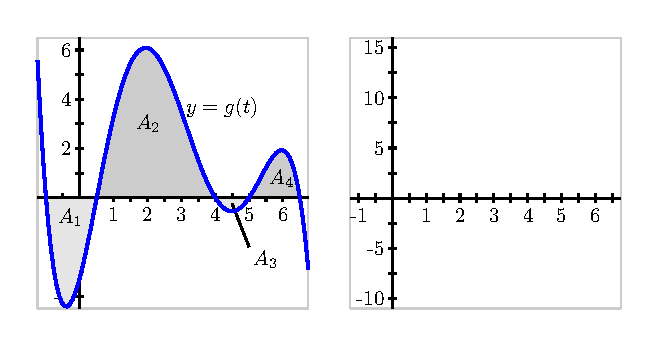
\includegraphics[scale=.75]{figures/5_2_Ez1.eps}

%ITEM
\item The tide removes sand from the beach at a small ocean park at a rate modeled by the function $$R(t) = 2 + 5\sin \left( \frac{4\pi t}{25} \right)$$
A pumping station adds sand to the beach at rate modeled by the function
$$S(t) = \frac{15t}{1+3t}$$
Both $R(t)$ and $S(t)$ are measured in cubic yards of sand per hour, $t$ is measured in hours, and the valid times are $0 \le t \le 6$.  At time $t = 0$, the beach holds $2500$ cubic yards of sand.

	\ba
		\item What definite integral measures how much sand the tide will remove during the time period $0 \le t \le 6$?  Why? 
		\item Write an expression for $Y(x)$, the total number of cubic yards of sand on the beach at time $x$.  Carefully explain your thinking and reasoning.
		\item At what instantaneous rate is the total number of cubic yards of sand on the beach at time $t = 4$ changing?  
		\item Over the time interval $0 \le t \le 6$, at what time $t$ is the amount of sand on the beach least?  What is this minimum value?  Explain and justify your answers fully.
	\ea
	
%ITEM
\item When an aircraft attempts to climb as rapidly as
possible, its climb rate (in feet per minute) decreases as altitude
increases, because the air is less dense at higher altitudes.
Given below is a table showing performance data for a certain
single engine aircraft, giving its climb rate at various altitudes, where  $c(h)$ denotes the climb rate of the airplane at an altitude $h$.

\begin{center}
\scalebox{.9}{
  \begin{tabular}{|c||c|c|c|c|c|c|}%%c|c|c|c|c|}
    \hline
    $h$ (feet)& $0$ & $1000$ & $2000$ & $3000$ & $4000$ & $5000$ \\%&6000&7000&8000&9000&10,000\\
    \hline
    $c$ (ft/min)& $925$ & $875$ & $830$ & $780$ & $730$ & $685$ \\%&635&585&535&490&440\\
    \hline
    \hline
    $h$ (feet)& $6000$ & $7000$ & $8000$ & $9000$ & $10,000$ &\\
    \hline
    $c$ (ft/min)& $635$ & $585$ & $535$ & $490$ & $440$ &\\
    \hline    
  \end{tabular}
} % end scalebox
\end{center}

 Let a new function $m$, that also depends on $h$, (say $y = m(h)$) measure
the number of minutes required for a plane at altitude $h$ to climb the
next foot of altitude.
\ba
	\item[a.] Determine a similar table of values for $m(h)$ and explain how it is related to the table above.  Be sure to discuss the units on $m$.

	\item[b.] Give a careful interpretation of a function whose derivative
is $m(h)$.  Describe what the input is and what the output is.  Also,
explain in plain English what the function tells us.

	\item[c.] Determine a definite integral whose value tells us exactly the number of minutes required for the airplane to ascend to
$10,000$ feet of altitude.  Clearly explain why the value of this integral has the required meaning.  

	\item[d.] Determine a formula for a function $M(h)$ whose value tells us the exact number of minutes required for the airplane to ascend to $h$ feet of altitude.

	\item[e.] Estimate the values of $M(6000)$ and $M(10000)$ as accurately as you can.  Include units on your results.
\ea
\end{enumerate}

\noindent{\bf In exercises 4--7, find $F'(x)$.}

\begin{enumerate}[1),resume]
\item $\ds F(x) = \int_2^{x^3+x} \frac{1}{t}\ dt$
\item $\ds F(x) = \int_{x^3}^{0} t^3\ dt$
\item $\ds F(x) = \int_{x}^{x^2} (t+2)\ dt$
\item $\ds F(x) = \int_{\ln x}^{e^x} \sin t\ dt$
\end{enumerate}

%------------------------------------------
% END OF EXERCISES ON FIRST PAGE
%------------------------------------------
\end{multicols*}
\end{adjustwidth*}

%\clearpage
%
%\begin{adjustwidth*}{}{-2.25in}
%\setlength{\columnsep}{25pt}
%\begin{multicols*}{2}\small
%
%\noindent{\bf In Exercises 69--72, an acceleration function of an object moving along a straight line is given. Find the change of the object's velocity over the given time interval.}
%
%\begin{enumerate}[1),start=69]
%\item $a(t) = -32$ ft/s$^2$ on $[0,2]$
%\item $a(t) = 10$ ft/s$^2$ on $[0,5]$
%\item $a(t) = t$ ft/s$^2$ on $[0,2]$
%\item $a(t) = \cos t$ ft/s$^2$ on $[0,\pi]$
%
%    \item A function $f$ is given piecewise by the formula
%  $$f(x) = \left\{ 
%  	\begin{array}{lr}
%	-x^2 + 2x + 1, & \ \mbox{if} \ 0 \le x < 2 \\
%	-x + 3, & \ \mbox{if} \ 2 \le x < 3 \\
%	x^2 - 8x + 15, & \ \mbox{if} \ 3 \le x \le 5
%	\end{array}
%	\right.
%  $$
%  \ba
%  	\item Determine the exact value of the net signed area enclosed by $f$ and the $x$-axis on the interval $[2,5]$.
%	\item Compute the exact average value of $f$ on $[0,5]$.
%	\item Find a formula for a function $g$ on $5 \le x \le 7$ so that if we extend the above definition of $f$ so that $f(x) = g(x)$ if $5 \le x \le 7$, it follows that $\int_0^7 f(x) \, dx = 0.$
%  \ea
%\end{enumerate}
%
%\begin{enumerate}[1),resume]
% \item The instantaneous velocity (in meters per minute) of a moving object is given by the function $v$ as pictured below.  Assume that on the interval $0 \le t \le 4$, $v(t)$ is given by $v(t) = -\frac{1}{4}t^3 + \frac{3}{2}t^2 + 1$, and that on every other interval $v$ is piecewise linear, as shown.
%
%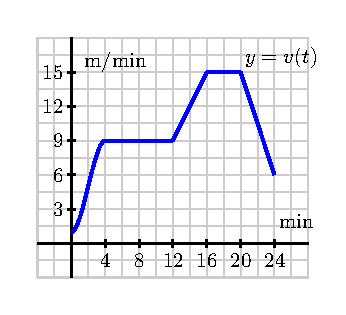
\includegraphics[scale=.75]{figures/4_4_Ez2.eps}
%
%    \ba
%  	\item Determine the exact distance traveled by the object on the time interval $0 \le t \le 4$.
%	\item What is the object's average velocity on $[12,24]$?
%	\item At what time is the object's acceleration greatest?
%	\item Suppose that the velocity of the object is increased by a constant value $c$ for all values of $t$.  What value of $c$ will make the object's total distance traveled on $[12,24]$ be 210 meters?
%  \ea
%  
%    \item When an aircraft attempts to climb as rapidly as
%possible, its climb rate (in feet per minute) decreases as altitude
%increases, because the air is less dense at higher altitudes.
%Given below is a table showing performance data for a certain
%single engine aircraft, giving its climb rate at various altitudes, where  $c(h)$ denotes the climb rate of the airplane at an altitude $h$.
%
%
%\begin{center}
%\scalebox{.85}{
%  \begin{tabular}{|c||c|c|c|c|c|c|}
%    \hline
%    $h$ (feet)&0&1000&2000&3000&4000&5000\\
%    \hline
%    $c$ (ft/min)&925&875&830&780&730&685\\
%    \hline
%    \hline
%    $h$ (feet)&6000&7000&8000&9000&10,000&\\
%    \hline
%    $c$ (ft/min)&635&585&535&490&440&\\
%    \hline
%  \end{tabular}
%  }
%\end{center}
%
%
% Let a new function called $m(h)$ measure
%the number of minutes required for a plane at altitude $h$ to climb the
%next foot of altitude.
%\ba
%	\item Determine a similar table of values for $m(h)$ and explain how it is related to the table above.  Be sure to explain the units.
%
%	\item Give a careful interpretation of a function whose derivative
%is $m(h)$.  Describe what the input is and what the output is.  Also,
%explain in plain English what the function tells us.
%
%	\item Determine a definite integral whose value tells us exactly the number of minutes required for the airplane to ascend to
%10,000 feet of altitude.  Clearly explain why the value of this integral has the required meaning.
%
%	\item Use the Riemann sum $M_5$ to estimate the value of the integral you found in (c).  Include units on your result.
%\ea
%
%
%\end{enumerate}
%
%%---------------------------------------------
%% END OF EXERCISES ON SECOND PAGE
%%---------------------------------------------
%\end{multicols*}
%\end{adjustwidth*}

\afterexercises